\begin{figure}[tb!]
\centering
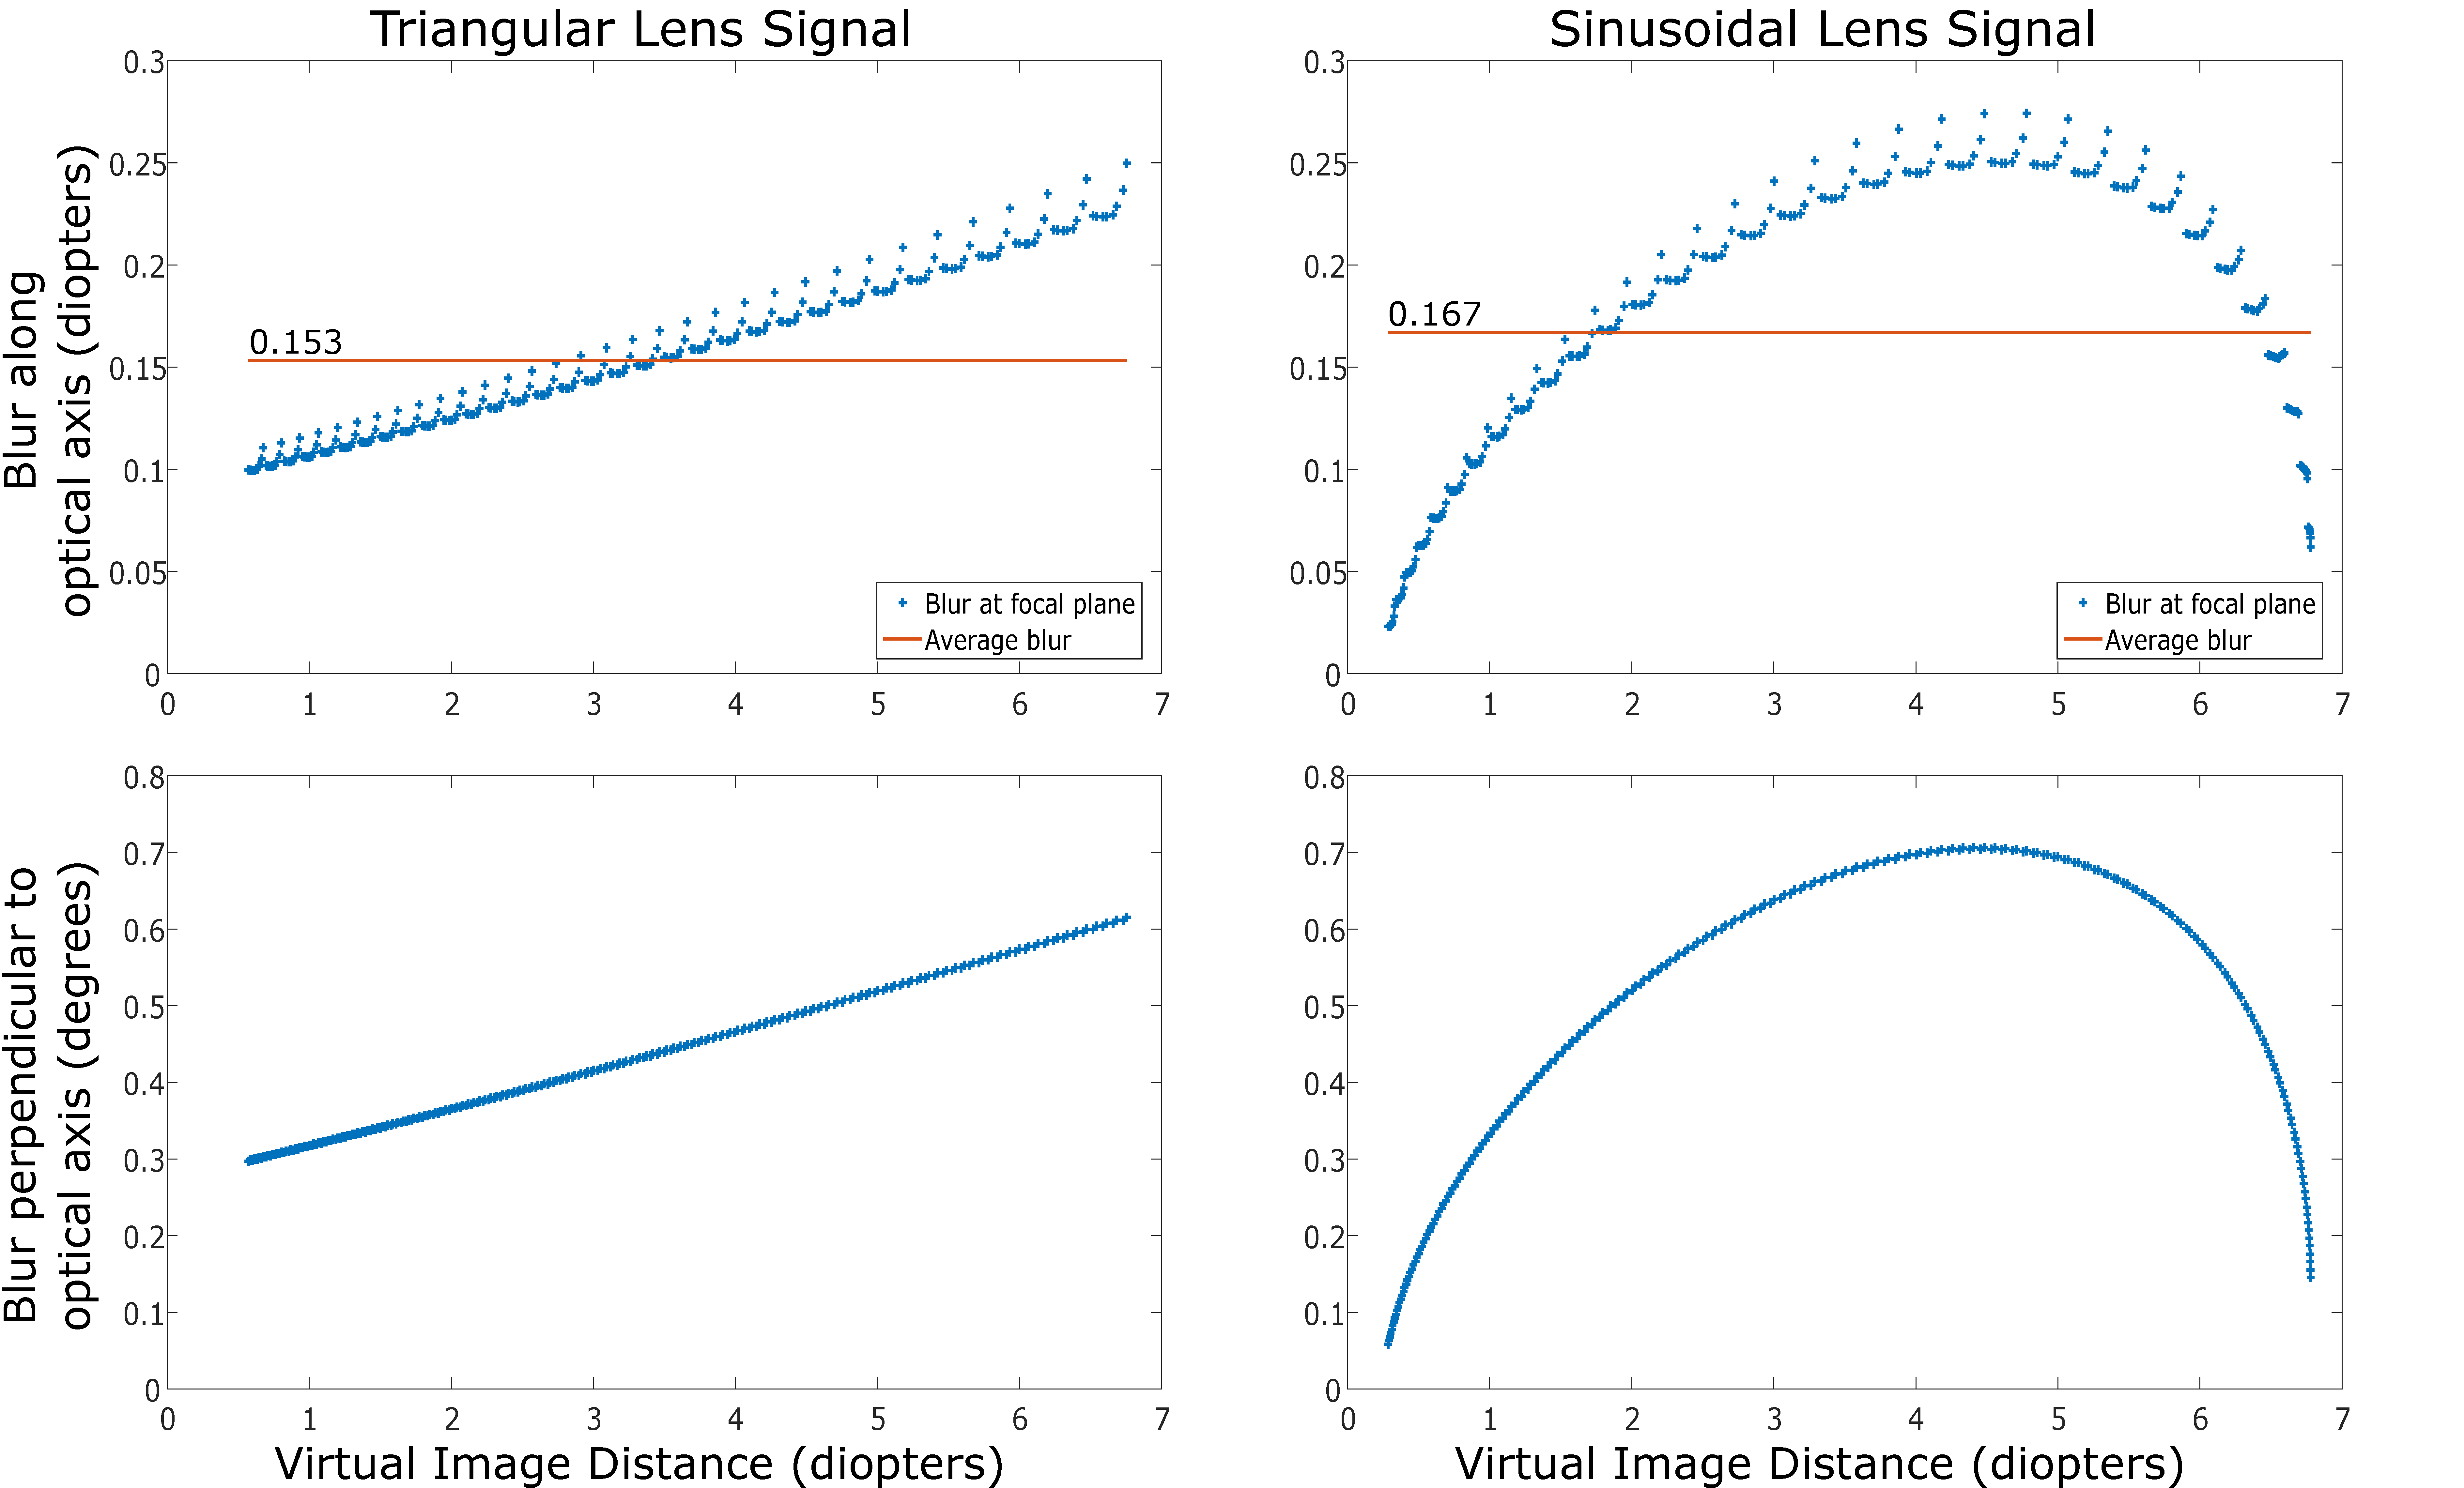
\includegraphics[width=\columnwidth]{images/volumetric/blur_graphs}
\caption[Volumetric NED: Longitudinal and lateral blur of voxels at each depth plane]{\emph{Top row: }Graphs indicate the depth blur for a color voxel at each depth plane and the average depth blur for color voxels of all depth planes. The depth blur arises because the rendering pipeline decomposes each color voxel to multiple single-color binary voxels, which are spread along the perspective projection lines. \emph{Bottom row: } The optics of our NED cause the FoV of the virtual image to slightly change over the lens cycle; this changing FoV is graphed. This creates a blur perpendicular to the optical axis leading to a loss in spatial resolution.}
\label{fig:volumetric:blur_graphs}
\end{figure}
    
    
